\documentclass[journal]{vgtc}                     % final (journal style)
%\documentclass[journal,hideappendix]{vgtc}        % final (journal style) without appendices
%\documentclass[review,journal]{vgtc}              % review (journal style)
%\documentclass[review,journal,hideappendix]{vgtc} % review (journal style)
%\documentclass[widereview]{vgtc}                  % wide-spaced review
%\documentclass[preprint,journal]{vgtc}            % preprint (journal style)


%% Uncomment one of the lines above depending on where your paper is
%% in the conference process. ``review'' and ``widereview'' are for review
%% submission, ``preprint'' is for pre-publication in an open access repository,
%% and the final version doesn't use a specific qualifier.

%% If you are submitting a paper to a conference for review with a double
%% blind reviewing process, please use one of the ``review'' options and replace the value ``0'' below with your
%% OnlineID. Otherwise, you may safely leave it at ``0''.
\onlineid{0}

%% In preprint mode you may define your own headline. If not, the default IEEE copyright message will appear in preprint mode.
%\preprinttext{To appear in IEEE Transactions on Visualization and Computer Graphics.}

%% In preprint mode, this adds a link to the version of the paper on IEEEXplore
%% Uncomment this line when you produce a preprint version of the article 
%% after the article receives a DOI for the paper from IEEE
%\ieeedoi{xx.xxxx/TVCG.201x.xxxxxxx}

%% declare the category of your paper, only shown in review mode
\vgtccategory{Research}

%% Paper title.
\title{Visual Analytics of Sailor Shift and Oceanus Folk}

%% Author ORCID IDs should be specified using \authororcid like below inside
%% of the \author command. ORCID IDs can be registered at https://orcid.org/.
%% Include only the 16-digit dashed ID.
\author{%
%   \authororcid{Josiah S.\ Carberry}{0000-0002-1825-0097},
%   Ed Grimley, and 
%   Martha Stewart
	CHEN Haitong, NIGEL-NICHOLAS, SU Wentao,\\
	XIAO liyin, and Zhou Xuan
}

\authorfooter{
  %% insert punctuation at end of each item
  \item
  	E-mail: 
  \item
  	E-mail: ed.grimley@example.com.

  \item 
  	E-mail: martha.stewart@example.com.
}

%% Abstract section.
\abstract{%
  Centering around synthetic data of Sailor Shift and Oceanus Folk Music Genre, we're building a visualization tool that can interpret influence from surface and deep level. Using the concept of influence, we also are able to make a prediction of who is going to be the next upcoming star from Oceanus Folk music.
}

%% Keywords that describe your work. Will show as 'Index Terms' in journal
%% please capitalize first letter and insert punctuation after last keyword
\keywords{Data Visualization, Influence Network, Prediction}

%% A teaser figure can be included as follows
% \teaser{
%   \centering
%   \includegraphics[width=\linewidth, alt={A view of a city with buildings peeking out of the clouds.}]{CypressView}
%   \caption{%
%   	In the Clouds: Vancouver from Cypress Mountain.
%   	Note that the teaser may not be wider than the abstract block.%
%   }
%   \label{fig:teaser}
% }

%% Uncomment below to disable the manuscript note
\renewcommand{\manuscriptnotetxt}{}

%% Copyright space is enabled by default as required by guidelines.
%% It is disabled by the 'review' option or via the following command:
%\nocopyrightspace


%%%%%%%%%%%%%%%%%%%%%%%%%%%%%%%%%%%%%%%%%%%%%%%%%%%%%%%%%%%%%%%%
%%%%%%%%%%%%%%%%%%%%%% LOAD PACKAGES %%%%%%%%%%%%%%%%%%%%%%%%%%%
%%%%%%%%%%%%%%%%%%%%%%%%%%%%%%%%%%%%%%%%%%%%%%%%%%%%%%%%%%%%%%%%

%% Tell graphicx where to find files for figures when calling \includegraphics.
%% Note that due to the \DeclareGraphicsExtensions{} call it is no longer necessary
%% to provide the the path and extension of a graphics file:
%% \includegraphics{diamondrule} is completely sufficient.
% \graphicspath{{figs/}{figures/}{pictures/}{images/}{./}} % where to search for the images

%% Only used in the template examples. You can remove these lines.
\usepackage{tabu}                      % only used for the table example
\usepackage{booktabs}                  % only used for the table example
\usepackage{lipsum}                    % used to generate placeholder text
\usepackage{mwe}                       % used to generate placeholder figures
\usepackage{ccicons}                   % package to be able to use icons from creative commons

%% We encourage the use of mathptmx for consistent usage of times font
%% throughout the proceedings. However, if you encounter conflicts
%% with other math-related packages, you may want to disable it.
\usepackage{mathptmx}                  % use matching math font
\usepackage{float}
\usepackage{graphicx}
\usepackage{subcaption}
\usepackage{array}

\begin{document}

%%%%%%%%%%%%%%%%%%%%%%%%%%%%%%%%%%%%%%%%%%%%%%%%%%%%%%%%%%%%%%%%
%%%%%%%%%%%%%%%%%%%%%% START OF THE PAPER %%%%%%%%%%%%%%%%%%%%%%
%%%%%%%%%%%%%%%%%%%%%%%%%%%%%%%%%%%%%%%%%%%%%%%%%%%%%%%%%%%%%%%%

%% The ``\maketitle'' command must be the first command after the
%% ``\begin{document}'' command. It prepares and prints the title block.
%% the only exception to this rule is the \firstsection command

\maketitle

\section{INTRODUCTION}
We are tackling on the VAST 2025 Mini Challenge 1 \cite{VASTChallenge2025MC1}. The problem centers around Sailor Shift and the Oceanus Folk genre in music. Sailor Shift is a global music superstar whose viral 2028 breakout propelled her native genre, Oceanus Folk, onto the world stage and boosted tourism to her home island. Since her early days in the band Ivy Echoes, she has built a highly successful solo career characterized by frequent collaborations aimed at elevating lesser-known artists. Her former bandmates have also thrived in the industry, collectively inspiring a new generation of Oceanus Folk musicians. Journalist Silas Reed is trying to understand Sailor Shift and Oceanus Folk music's rise through the use of data visualization.

In the challenge, we're asked to solve 3 main tasks including a list of sub-tasks that guides how we can break down the data to find insights. This will be discussed in section \ref{sec:requirements}.

% \section{RELATED WORK}
% \subsection{Knowledge Graph Visualization}
% \subsection{Music Information Visualization}
% \subsection{Visual Analytics for Temporal and Network Data}


\section{DATA DESCRIPTION}

\subsection{Overview}
There is a dedicated public Github repository that hosts the data needed for the challenge \cite{vast2025mc1_data} in a zipped file. Once unpacked, there will be a .json file along with some descriptions on the data. Note that the data is completely synthetic and therefore any name resemblance to the real world is pure coincidental. The json file is processed via NetworkX \cite{networkx_multidigraph} and later on passed on to the visualization layer.

The given data provided is \textbf{Multi-directed graph} consisting of \textbf{17,412 nodes} and \textbf{37,857 edges}. The nodes and edges are differentiated by types (i.e. Node Type and Edge Type). Following are a breakdown of the distribution of node and edge types within the network.

\begin{figure}[H]
    \centering
    \includegraphics[width=0.4\textwidth]{node_type_distribution.png}
    \caption{Node Type distribution}
\end{figure}

\begin{figure}[H]
    \centering
    \includegraphics[width=0.4\textwidth]{edge_type_distribution.png}
    \caption{Edge Type distribution}
\end{figure}

For each node and edge type, there might be some extra attributes tied to the node.

\subsection{Nodes}
Node-specific attributes vary by \texttt{Node Type}. Persons may carry \texttt{name} and optional \texttt{stage\_name}. Musical groups and record labels carry identifying names (the schema text uses \texttt{name} or \texttt{Name} for organizations). Songs and albums support \texttt{genre} where applicable, Boolean \texttt{notable} chart prominence, string \texttt{release\_date} (year), optional \texttt{written\_date}, optional \texttt{notoriety\_date}, and for songs an optional Boolean \texttt{single} indicating standalone release versus inclusion on a larger album.

\subsection{Edges}

\begin{table}[htbp]
  \centering
  \small
  \caption{Directed edge types and node types involved}
  \label{tab:edges}
  \begin{tabular}{@{}>{\raggedright\arraybackslash}p{0.30\linewidth}>{\raggedright\arraybackslash}p{0.62\linewidth}@{}}
    \toprule
    \textbf{Edge type} & \textbf{Interpretation (source $\rightarrow$ target)} \\
    \midrule
    \multicolumn{2}{@{}l}{\textit{Creative roles on works}} \\
    \texttt{PerformerOf} & Person or group performed the song or album. \\
    \texttt{ComposerOf} & Person composed the song or album. \\
    \texttt{ProducerOf} & Person or label contributed to production of a song, album, person, or group. \\
    \texttt{LyricistOf} & Person wrote lyrics for the song or album. \\
    \texttt{MemberOf} & Person is or was a member of the musical group. \\
    \midrule
    \multicolumn{2}{@{}l}{\textit{Recording and distribution}} \\
    \texttt{RecordedBy} & Song or album was recorded with involvement of the record label (target). \\
    \texttt{DistributedBy} & Song or album was distributed with involvement of the record label (target). \\
    \midrule
    \multicolumn{2}{@{}l}{\textit{Inter-work and stylistic relations among songs and albums}} \\
    \texttt{InStyleOf} & Source work was performed partly in the style of the target (work, album, person, or group). \\
    \texttt{InterpolatesFrom} & Source work interpolates melodic material from the target work. \\
    \texttt{CoverOf} & Source work is a cover of the target work. \\
    \texttt{LyricalReferenceTo} & Source work makes a lyrical reference to the target work. \\
    \texttt{DirectlySamples} & Source work reuses recorded audio from the target via sampling. \\
    \bottomrule
  \end{tabular}
\end{table}

\section{TASK REQUIREMENTS}
\label{sec:requirements}

This project aims to develop visual analytics tools for exploring a music knowledge graph about Sailor Shift, Oceanus Folk, and the spread of musical influence. The system should help Silas Reed investigate Sailor's career, trace how Oceanus Folk expanded into the wider music world, and identify patterns that characterize rising stars.

The project requirements are summarized as follows:

\begin{itemize}
    \item \textbf{Task 1: Sailor Shift's career profile.} \\
    The system should support the exploration of Sailor Shift's artistic development, including who influenced her over time, who she collaborated with, and whom she directly or indirectly influenced. It should also reveal the nature of her influence to the Ocean Folk community.

    \item \textbf{Task 2: Diffusion of Oceanus Folk.} \\
    The visualizations should show whether Oceanus Folk's influence was intermittent or gradually rising. They should identify the genres and top artists most influenced by Oceanus Folk, while also examining how Oceanus Folk itself changed after Sailor's rise and which genres contributed to its contemporary inspiration.

    \item \textbf{Task 3: Rising star characterization.} \\
    The system should compare the careers of three artists in terms of popularity, influence, and career development. Based on this comparison, it should summarize common traits of rising stars and predict potential future Oceanus Folk stars over the next five years.
\end{itemize}

\section{VISULAIZATION DESIGN}
\subsection{System Overview}

As the requirements of the 3 tasks are very different from one another in terms of scale and aim, we design separate visualizations for each of the task.


\subsection{Sailor Shift Career Timeline}
To provide more context into Sailor Shift's career, here are some insights and trends about her work over the years.


\subsection{Influence and Collaboration Network}
\textbf{Task 1b / 1c / 2b}

\textbf{2b}\\
The influence and collaboration network was designed to identify the artists and genres most strongly connected to Oceanus Folk. The system first identifies Oceanus Folk songs and albums, then extracts related artists through creative relations such as \texttt{PerformerOf}, \texttt{ComposerOf}, \texttt{LyricistOf}, and \texttt{ProducerOf}. It then detects influence relations using edge types such as \texttt{InStyleOf}, \texttt{InterpolatesFrom}, \texttt{CoverOf}, \texttt{LyricalReferenceTo}, and \texttt{DirectlySamples}.

In this view, Oceanus Folk is placed as the central node, connected to influenced artists and genres. Node size represents either \texttt{influence\_weight} or \texttt{total\_signal}, while edge colors distinguish influence, collaboration, and combined influence-collaboration relations. The interactive version supports filtering by node category, relation type, edge weight, influence weight, and node count.
\begin{figure}[H]
    \centering
    \includegraphics[width=0.4\textwidth]{report_fig_q2b_network.png}
    \caption{Influence and collaboration network centered on Oceanus Folk.}
\end{figure}

\subsection{Oceanus Folk Diffusion}
\textbf{Task 2a/2c}

\textbf{2a} The Oceanus Folk diffusion view addresses whether the genre's influence was intermittent or gradually rising. The system aggregates influence relations by year and computes several metrics, including yearly influenced works, cumulative influenced works, influence events, unique affected artists, and unique affected genres.

The visualization combines yearly influenced works, a three-year moving average, cumulative growth, and influence event counts. This design allows short-term fluctuations and long-term diffusion to be examined together. The interactive dashboard also provides time presets, peak-year annotation, and change-point markers.

\begin{figure}[H]
    \centering
    \includegraphics[width=0.4\textwidth]{report_fig_q2a_trend.png}
    \caption{Temporal diffusion of Oceanus Folk influence.}
\end{figure}

\textbf{2c} In Task 2(c), we examine how Oceanus Folk changed with the rise of Sailor Shift. We use a line chart to show the yearly percentage of songs associated with Oceanus Folk. Using percentage instead of raw counts helps normalize yearly differences in the total number of released songs, making the comparison more reliable. The chart also divides the timeline into the periods before and after Sailor Shift's rise, with an average reference line as a baseline.

\begin{figure}[H]
    \centering
    \includegraphics[width=0.4\textwidth]{report_fig_q2c_trend.png}
    \caption{Oceanus Folk share among songs released each year}
\end{figure}

% The result shows that before Sailor Shift became famous, Oceanus Folk remained at a relatively low share with only small fluctuations. After around 2030, its share increases clearly and reaches several peaks. This suggests that Sailor Shift's rise helped reactivate Oceanus Folk, making it more visible and more frequently used in later music production.


\subsection{Genre Influence Flow}
\textbf{Task 2b / 2c}

\textbf{2b}
The genre influence flow view focuses on how different types of influence contributed to the spread of Oceanus Folk over time. It uses a theme river visualization based on yearly counts of five influence relations: \texttt{InStyleOf}, \texttt{InterpolatesFrom}, \texttt{CoverOf}, \texttt{LyricalReferenceTo}, and \texttt{DirectlySamples}.

Each stream represents one influence type, and its thickness shows the number or share of events in each year. This makes it possible to compare whether the spread was mainly driven by stylistic imitation, covers, sampling, interpolation, or lyrical references.

\begin{figure}[h]
    \centering
    \includegraphics[width=0.4\textwidth]{report_fig_q2a_theme_river.png}
    \caption{Theme river showing the composition of Oceanus Folk influence types over time.}
\end{figure}

The genre-level ranking further supports this analysis by identifying the genres most influenced by Oceanus Folk. In the current results, genres such as Dream Pop, Indie Folk, Desert Rock, Space Rock, and Synthwave show strong influence or collaboration signals.

\begin{figure}[h]
    \centering
    \includegraphics[width=0.4\textwidth]{report_fig_q2b_top_entities.png}
    \caption{Top genres and artists connected to Oceanus Folk influence.}
\end{figure}

\textbf{2c} To further analyze the contemporary inspiration sources of Oceanus Folk, we have designed two complementary charts: a stacked bar chart and a Sankey diagram. 

The stacked bar chart is used to display the composition structure of the sources of inspiration for Oceanus Folk in different years. Each bar represents a year, and the different colored parts within the bars represent different source genres. This chart is suitable for comparing the changes in the proportion of inspiration sources between different years. Through this chart, we can observe whether Oceanus Folk always relies on a fixed few genres or gradually incorporates new musical elements. 

The Sankey diagram further emphasizes the flow relationships between different genres. The stacked bar chart answers the question "How much did each genre contribute in each year", while the Sankey diagram answers the question "Where did these inspirations come from and how did they flow to Oceanus Folk". This is particularly important for Task 2(c), as the problem essentially focuses on directional influence. The Sankey diagram can more clearly display the flow path from the source genre to Oceanus Folk, making the process of music evolution more intuitive. 

\begin{figure}[h]
    \centering

    \begin{subfigure}{0.48\columnwidth}
        \centering
        \includegraphics[width=\textwidth]{image_2.png}
		\caption{Stacked bar chart}
        \label{fig:stacked_bar}
    \end{subfigure}
    \hfill
    \begin{subfigure}{0.48\columnwidth}
        \centering
        \includegraphics[width=\textwidth]{image.png}
        \caption{Sankey diagram}
        \label{fig:sankey}
    \end{subfigure}

    \caption{Contemporary inspiration sources of Oceanus Folk.}
    \label{fig:small_two_images}
\end{figure}

% When these two graphs are combined, we find that Oceanus Folk is increasingly drawing inspiration from emerging genres. This indicates that the development of Oceanus Folk is a two-way influence process: on the one hand, it spreads outward and influences other genres; on the other hand, it also absorbs elements from new musical styles. Therefore, the contemporary evolution of Oceanus Folk is not simply a continuation of tradition, but rather constantly changes under the combined influence of Sailor Shift's popularity and emerging styles.

\subsection{Rising Star Comparison}
\textbf{Task 3a / 3b}
The third Mini-Challenge task departs from descriptive analytics, which asks what happened inside Oceanus Folk, and demands predictive analytics, which asks who will rise next. Predictive questions impose a particular visualisation design problem: the answer is a forecast, but every encoding the reader sees is built from historical evidence, so the reader must be able to inspect both the forecast and the chain of evidence behind it. A black-box prediction would defeat the purpose of a visual-analytics deliverable.

Our approach therefore centres on a five-step pipeline that bridges historical benchmarking with forward forecasting. Three baseline superstars supply the reference profiles; six rising-star dimensions are computed for every eligible candidate; a multiplicative composite collapses these into a single score; and a final composite landscape positions the top picks. The five steps trace, in order, what each candidate did, who they are connected to, how their dimension profile compares against peers, how those dimensions aggregate into a forward signal, and where they sit on the predictive landscape relative to the baselines.

\subsubsection{Addressing Temporal Dynamics in Static Visualizations}
\label{sec:time_dim_viz_motivation}
A central design tension in this task is that the prediction call lives at the cross-section, that is, who is rising right now, while the underlying evidence is longitudinal. Radar profiles and ranked scatter plots are excellent for snapshot comparison, but a snapshot alone discards the very signal we want to detect: a derivative, not a level. To remain faithful to Munzner's principle that the visual encoding must serve the task abstraction, we therefore absorb the time axis into the feature-engineering layer rather than relying on the final marks to carry it. Three of the six rising-star dimensions used by Step 3 and Step 4 are intrinsically temporal:

\begin{itemize}
    \item \textbf{OF Momentum} quantifies output velocity. The activity intensity in the most recent three-year window is compared against the artist's earlier baseline, producing a slope-of-growth signal that is positive only when the artist is genuinely accelerating relative to themselves.
    \item \textbf{Trajectory Acceleration} measures career burstiness through a discrete second-derivative on output: release frequency in the second half of an artist's history is contrasted with release frequency in the first half, so a flat career and an exponential one are clearly separated.
    \item \textbf{Recency Weighting} applies an exponential decay to artists whose last release is far from the dataset's present, ensuring the model favours forward-looking signatures over historical icons.
\end{itemize}

The pipeline that follows operationalises these features into a single composite score. \Cref{sec:time_dim_viz} returns to them visually, on a time axis, so that the temporal reasoning embedded in the score is recoverable from the figure rather than buried inside an opaque scalar.

\subsubsection{The 5-Step Pipeline Implementation}
We implement custom graph rendering with D3.js and multi-dimensional interactive filtering with Plotly.js. The workflow proceeds in five stages, each motivated by the visual-analytics design principle that the encoding chosen at every stage should serve the task abstraction of that stage. The first four stages are described here; Step 5 lives in the case study (\cref{sec:step5_landscape}) because it answers a question that only becomes meaningful once Steps 1--4 have produced their primitives.

\textbf{Step 1: Career Timelines.}
For each candidate we plot annual song output and the rolling notable-work ratio on a shared calendar axis. The visual encoding is deliberately conservative: bar marks for counts and a line mark for the ratio, both on linear scales, because the analyst's task here is browsing for consistent performers, and any aesthetic flourish would only obscure inter-artist comparison. The chart is the discriminator between a one-hit wonder and an artist with sustained output, the latter being a necessary precondition for entering the rising-star pool.
\begin{figure}[H]
    \centering
    \includegraphics[width=0.48\textwidth]{Career Timeline Analysis.png}
    \caption{Step 1: career trajectories that separate consistent quality from one-hit wonders.}
    \label{fig:step1}
\end{figure}

\textbf{Step 2: Influence Network.}
The second view answers a connectivity question that the bar chart of Step 1 cannot: does the candidate's reach extend beyond their immediate collaborators? We render a force-directed layout with the candidate at the centre and the influenced artists radiating outward; node size encodes the number of influenced works and edge weight encodes relation count. This is the visualisation of industry gravity, the property that distinguishes a productive but isolated artist from a productive hub.
\begin{figure}[H]
    \centering
    \includegraphics[width=0.4\textwidth]{Influence Network.png}
    \caption{Step 2: influence network and core industry hubs.}
    \label{fig:step2}
\end{figure}

\textbf{Step 3: Radar Profiles.}
Step 3 condenses the six rising-star dimensions into a radar layout: Momentum, Quality, Reach, Bridge, Network, and Traction. Each axis is independently rank-percentile-normalized within the candidate pool so that every dimension spans 0 to 1, which lets the reader compare the shape of the polygon, rather than absolute magnitude, across candidates. A balanced polygon signals a balanced profile, while a long spike indicates an artist who is exceptional on one axis but vulnerable on others.
\begin{figure}[H]
    \centering
    \includegraphics[width=0.4\textwidth]{Rising Star Analysis Workbench.png}
    \caption{Step 3: the Analysis Workbench using radar profiles to visualise the "Star DNA".}
    \label{fig:step3}
\end{figure}

\textbf{Step 4: Prediction Algorithm.}
Step 4 collapses the radar into a single rising-star score through a multiplicative composite that draws on the Cobb--Douglas form. The core factor is the geometric mean of the weighted dimension sum and a forward-trend index, modulated by a profile-coherence term and a breadth multiplier, and finally damped by an exponential recency-decay penalty. The multiplicative structure is the key methodological choice: a candidate strong on only one axis cannot compensate via another, because multiplication by a small factor cannot be cured by addition. The diagram in \cref{fig:step4} traces the weights and the order of combination.
\begin{figure}[H]
    \centering
    \includegraphics[width=0.48\textwidth]{Rising Star Prediction Algorithm.png}
    \caption{Step 4: logic and weighting of the predictive scoring model.}
    \label{fig:step4}
\end{figure}

\subsubsection{Time-Dimension Visualization: Composite Score Evolving Over a Career}
\label{sec:time_dim_viz}
The pipeline of Steps 1--4 produces a single scalar per artist, and that scalar by construction collapses the temporal information motivated in \cref{sec:time_dim_viz_motivation} back into a snapshot. The radar profile and the score landscape both inherit this property: they are cross-sectional encodings of an intrinsically longitudinal quantity. To restore the time axis on the page without abandoning the composite, we re-run the same scoring pipeline at every career age, using only the data that would have been observable up to that age. The candidate pool, the percentile normalisation, the geometric trend index, and the multiplicative composite are all evaluated under the same age-truncation rule, so the value on the curve at career age $a$ is exactly what the project pipeline would have output had the dataset been frozen at that snapshot.

Each artist's calendar timeline is then shifted so that age $0$ aligns with their first Oceanus Folk release. This alignment is borrowed from cohort analysis in time-series visualization and has a clear analytical purpose: artists with very different debut years can be compared by growth slope rather than by absolute year, which is the geometric equivalent of asking how steeply each artist rose during the same career stage. A static figure is included for the paper, and an interactive D3.js companion at \texttt{trajectory\_tails.html} supports per-point tooltips and group toggles so that an analyst can isolate any subset of the entities for closer inspection.

The chart in \cref{fig:trajectory} traces the seven entities the project pipeline singles out. The three baseline superstars are Sailor Shift, the protagonist of the data set; Embers of Wrath, automatically selected as the Influence Magnet archetype by the comparison rules; and Orla Seabloom, automatically selected as the Rapid Riser archetype. Ivy Echos appears as a dashed grey arc for narrative context: it is Sailor Shift's former band and is formally excluded from the prediction pool because Sailor's bandmates are correlated co-collaborators rather than independent candidates. The remaining three are the top-ranked predicted rising stars Copper Canyon Ghosts, Daniel O'Connell, and Beatrice Albright. A candidate is credible as a rising star when, at the same career age as Sailor Shift, their composite sits at or above Sailor Shift's confirmed end-of-career level, marked here by the dashed horizontal reference.

\begin{figure}[H]
    \centering
    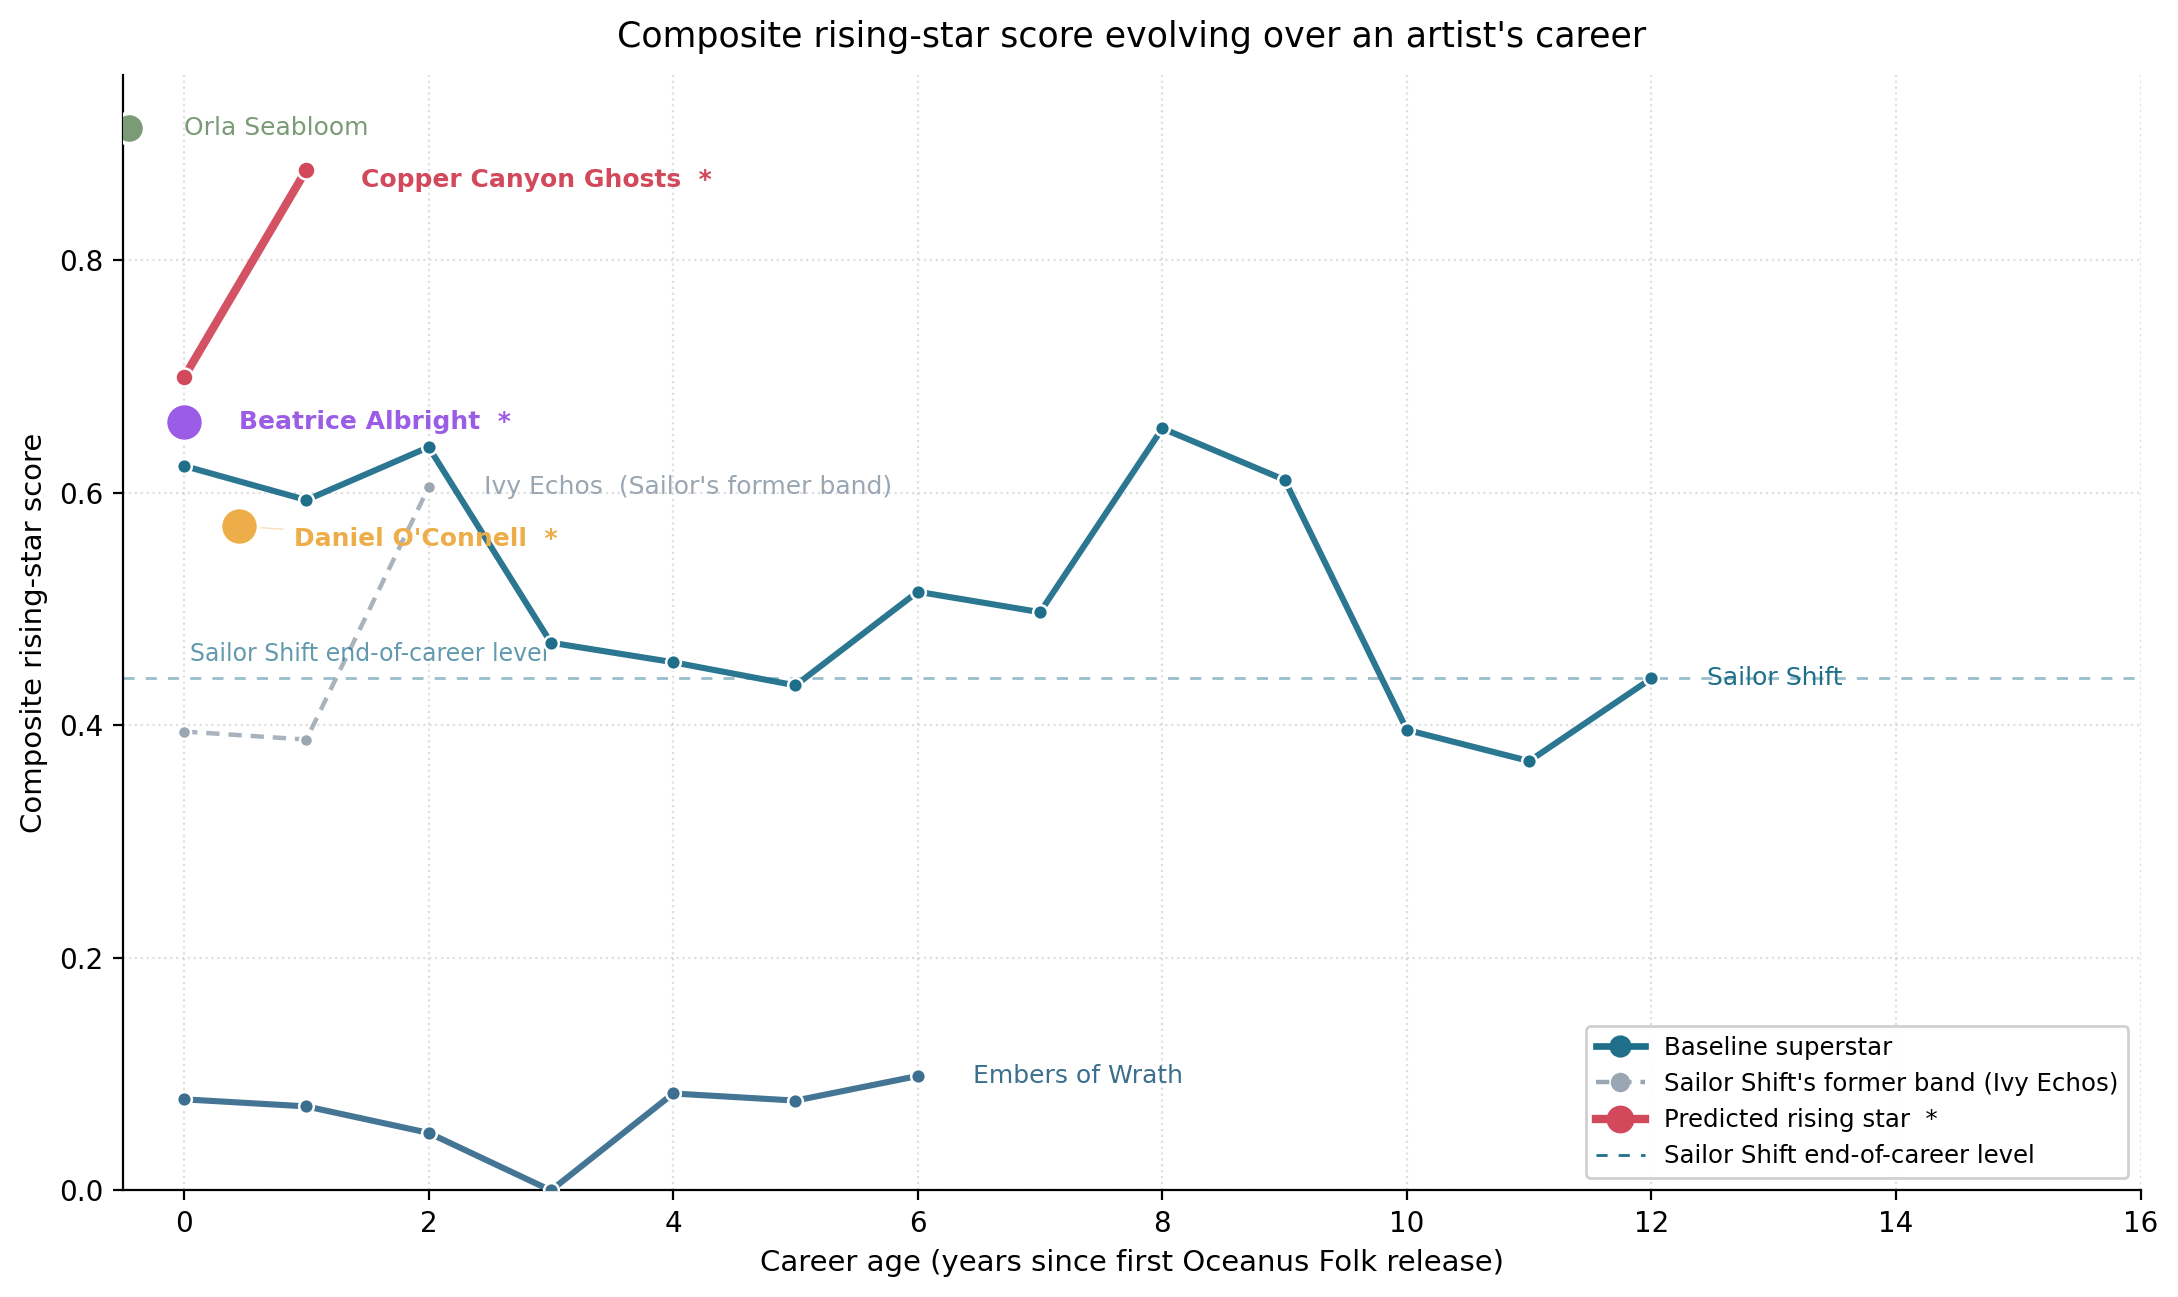
\includegraphics[width=0.48\textwidth]{../viz/report_fig_t_trajectory.png}
    \caption{Composite rising-star score traced over career age for the seven entities highlighted by the project pipeline. Sailor Shift, Embers of Wrath, and Orla Seabloom anchor the comparison as the three baseline archetypes; Ivy Echos appears as a dashed grey arc, supplying narrative context as Sailor Shift's former band just before her 2028 breakout. The three predicted rising stars sit above Sailor Shift's confirmed end-of-career level, marked by the dashed horizontal reference, at their actual career ages, which is the visual basis for their placement in the top-right quadrant of \cref{fig:step5}. Embers of Wrath's persistently low curve underscores that high incoming influence alone, in the absence of forward Momentum or Recency, does not earn a rising-star score under the model.}
    \label{fig:trajectory}
\end{figure}

\section{CASE STUDY}
\subsection{Sailor Shift's Career Profile}
\textbf{Task1}
\subsection{The Spread of Oceanus Folk}
\textbf{Task2}

The results suggest that Oceanus Folk influence developed through both gradual accumulation and intermittent bursts. The diffusion view shows influenced works from \textbf{2007 to 2038}, with the cumulative number reaching \textbf{149}. This indicates that the genre had a sustained impact over several decades.The strongest peak occurs in \textbf{2027}, with \textbf{25 influenced works} and \textbf{39 influence events}. Since Sailor Shift’s global breakthrough happened in 2028, this peak suggests that Oceanus Folk’s influence was already increasing before her worldwide success, and her rise likely accelerated an existing diffusion process.The network and ranking views show that Oceanus Folk influenced a diverse range of genres. The strongest genre signals appear in \textbf{Dream Pop}, \textbf{Indie Folk}, \textbf{Desert Rock}, \textbf{Space Rock}, and \textbf{Synthwave}. This indicates that Oceanus Folk spread beyond traditional folk contexts and entered both folk-adjacent and more experimental popular styles.At the artist level, highly influenced entities include \textbf{Blazing Collective}, \textbf{Jonathan Diaz}, \textbf{Ming Zhao}, \textbf{Xiuying Xie}, and \textbf{Xiuying Yao}. Some artists show stronger influence weights, while others are more prominent through collaboration weights, suggesting that Oceanus Folk spread through both stylistic influence and direct creative partnerships.Overall, the visual evidence shows that Oceanus Folk did not spread in a purely linear way. Instead, it expanded through repeated bursts of attention, long-term cumulative growth, and cross-genre collaboration.

\subsection{The Evolution of Oceanus Folk}
\textbf{Task2}
Overall, the visualizations suggest that the rise of Sailor Shift not only increased the visibility of Oceanus Folk, but also changed its role in the contemporary music ecosystem. 

Before Sailor Shift became famous, Oceanus Folk accounted for only a small share of yearly released songs, with limited fluctuations. However, after around 2030, its share increases noticeably and reaches several peaks, indicating that the genre was reactivated and more frequently used in later music production. 

At the same time, the stacked bar chart and Sankey diagram show that Oceanus Folk increasingly draws inspiration from other genres rather than remaining a fixed traditional style. In particular, its contemporary development is connected with more modern and cross-genre styles such as Synthwave, Dream Pop, and Desert Rock, while also maintaining links with folk-related genres such as Indie Folk and Americana. 

This suggests a two-way influence process: Oceanus Folk spreads outward and influences other genres, but it also absorbs new musical elements from emerging styles. Therefore, the contemporary evolution of Oceanus Folk is not simply a continuation of tradition, but a dynamic transformation shaped by both Sailor Shift's popularity and the broader diversification of musical genres.
\subsection{Characterizing Rising Stars}
\textbf{Task3}
Our analysis culminates in the identification of specific patterns that characterize upcoming superstars in Oceanus Folk.

\subsubsection{Benchmark Insights}
The three baseline superstars are not picked arbitrarily. They are returned by the comparison rules in the project pipeline as three deliberately different archetypes, and the contrast between them is what allows the model to define a balanced rising-star profile by triangulation.

Sailor Shift is the balanced archetype. Across her 13-year arc she sustains non-trivial Momentum, Quality, and Breadth simultaneously, and her composite trajectory in \cref{fig:trajectory} oscillates in the $0.37$--$0.66$ band, peaks at age $8$, and settles at her published value of $0.44$. The model treats this profile as the canonical signature of a sustained superstar.

Embers of Wrath illustrates the Influence Magnet failure mode. The group accumulates an unusually high incoming-influence count of $30$, yet its composite stays below $0.10$ throughout its active years. The lesson is that reception of influence, in the absence of recent Momentum or output Acceleration, does not register as rising-star potential. A score model that rewarded inward influence linearly would have mis-ranked this entity; the multiplicative composite correctly identifies the missing forward signal.

Orla Seabloom is a Rapid Riser whose career so far is a single-year burst of seven notable songs. She therefore reaches the highest age-$0$ composite of any tracked artist, approximately $0.91$, yet her trajectory contains only one data point. This is the visual signature of a one-year wonder, and the breadth multiplier in Step 4 is precisely designed to discount this profile until a longitudinal track record emerges.

Taken together, the three baselines define the criterion a credible rising-star candidate must satisfy: recent Momentum that Embers of Wrath lacks, sustained Quality that a transient burst cannot provide, and at least incipient longitudinal Breadth that distinguishes a continuing career from a one-year wonder.

\subsubsection{Step 5: Composite Score Landscape and Predictions}
\label{sec:step5_landscape}
With the balance criterion in hand, Step 5 visualises every eligible candidate as a point in a two-dimensional landscape. The horizontal axis carries Future Trend, a Cobb--Douglas-style geometric blend of Momentum, Recency, Acceleration, and Breadth; the vertical axis carries Historical Strength, defined as the percentile-weighted sum across the six radar dimensions. The choice of a scatter plot follows directly from the data abstraction: each candidate is a vector in a forward-potential versus past-accomplishment plane, and a bivariate quantitative pair maps most expressively to position on perpendicular axes, which is the highest-ranked encoding for quantitative data in the standard visualization-channel hierarchy.

The geometric reading of the chart is straightforward. The upper-right quadrant is precisely where both percentiles are high simultaneously, and this co-occurrence is the geometric translation of the multiplicative core inside the composite formula: a candidate cannot reach the corner without satisfying both axes at once, because the square-root of the product collapses whenever either factor is small. The lower-left quadrant is the failure zone, where both criteria are weak; the two off-diagonal quadrants house the asymmetric archetypes the benchmark insights warned against.

\begin{figure}[H]
    \centering
    \includegraphics[width=0.48\textwidth]{Composite Score Landscape.png}
    \caption{Step 5: composite landscape identifying the top three predicted stars in the upper-right quadrant.}
    \label{fig:step5}
\end{figure}

\Cref{fig:step5} surfaces three artists that lead the pack by combining established mastery with the highest forward Momentum. Their selection is consistent with the three failure modes derived in the benchmark insights and traceable to specific evidence in the composite trajectory of \cref{fig:trajectory}.

Copper Canyon Ghosts leads on Industry Traction and OF Momentum. It is the only candidate whose composite trajectory in \cref{fig:trajectory} shows an upward slope across multiple years, climbing from $0.74$ at age $0$ to $0.88$ at age $1$. Daniel O'Connell exhibits exceptional Quality signals and Quality consistency, supplying the sustained-Quality criterion the Embers of Wrath counter-example warned against violating. Beatrice Albright acts as a hub in the influence network with strong collaborative ties, supplying the active outward-influence ingredient that pure-reception archetypes lack. Each prediction therefore rests on a specific dimension that the benchmark superstars either embodied or conspicuously failed to embody, which means the prediction is auditable rather than opaque.

\subsubsection{Conclusion}
The prediction pipeline succeeds because it treats slope and acceleration as first-class signals rather than reducing every artist to a cumulative total. This is a design choice motivated by a visual-analytics principle that runs through the entire challenge: the question being asked must drive the encoding being shown, and a static dashboard cannot answer a question about rate of change no matter how polished the static encoding is. Visualising the composite trajectory across career age in \cref{fig:trajectory} lets the reader audit the temporal reasoning frame by frame, verify that every predicted candidate already exceeds Sailor Shift's end-of-career level at their actual career age, and trace each decision back through Steps 1--5 to the underlying yearly data. The resulting prediction is not a black-box scalar; it is a defensible, evidence-aligned forecast that satisfies the dual requirement of Task 3, namely characterising rising stars and identifying who will be next.
\section{CONCLUSION}



% \firstsection{Introduction}

% \maketitle


%% \section{Introduction} %for journal use above \firstsection{..} instead
% This template is for papers of VGTC-sponsored conferences such as IEEE VIS, IEEE VR, and ISMAR which are published as special issues of TVCG.
% The template does not contain the respective dates of the conference/journal issue, these will be entered by IEEE as part of the publication production process.
% Therefore, \textbf{please leave the copyright statement at the bottom-left of this first page untouched}.


% \section{Author Details}

% You should specify ORCID IDs for each author (see \url{https://orcid.org/}  to register) for disambiguation and long-term contact preservation.
% Use \verb|\authororcid{Author Name}{0000-0000-0000-0000}| for each author, replacing the ``Author Name'' and using the 16-digit (hyphenated) ORCID ID for the second parameter.
% The template shows an example without ORCID IDs for two of the authors.
% ORCID IDs should be provided in all cases.

% Each author's affiliations have to be provided in the author footer on the bottom-left corner of the first page.
% It is permitted to merge two or more people from the same institution as long as they are shown in the same order as in the overall author sequence on the top of the first page.
% For example, if authors A, B, C, and D are from institutions 1, 2, 1, and 2, respectively, then it is ok to use 2 bullets as follows:
% \begin{itemize}
%   \item A and C are with Institution 1. E-mail: \{a\,$|$\,c\}@i1.com\,.

%   \item B and D are with Institution 2. E-mail: \{b\,$|$\,d\}@i2.org\,.
% \end{itemize}


% \section{Hyperlinks and Cross References}

% The style uses the \verb|hyperref| package which can typeset clickable hyperlinks using \verb|\href{...}{...}|, hyperlinked URLs using \verb|\url{...}|, and turns references into internal links.

% The style also uses \verb|cleveref| to automatically and consistently format cross references.
% We recommend that you use the \verb|\cref{label}| and \verb|\Cref{label}| calls instead of \verb|Figure~\ref{label}| or similar.
% \verb|\Cref| should be used when starting a sentence to spell out the reference (e.g.\ ``Section'') while \verb|\cref| should be used when referencing within a sentence to abbreviate (e.g.\ ``Sec.'').
% Here are examples for use within a sentence: \cref{fig:vis_papers}, \cref{tab:vis_papers}, \cref{sec:supplement_inst,sec:references_inst}, \cref{eq:sum}.
% The following sentences all start with a reference, so use \verb|\Cref|.
% \Cref{fig:vis_papers} is a \verb|figure| environment.
% \Cref{tab:vis_papers} is a \verb|table| environment.
% \Cref{sec:supplement_inst,sec:references_inst} are \verb|section| environments.
% \Cref{eq:sum} is an \verb|equation| environment.


% \section{Figures}

% \subsection{Loading figures}

% The style automatically looks for image files with the correct extension (eps for regular \LaTeX; pdf, png, and jpg for pdf\LaTeX), in a set of given subfolders defined above using \verb|\graphicspath|: figures/, pictures/, images/.
% It is thus sufficient to use \verb|\includegraphics{CypressView}| (instead of \verb|\includegraphics{pictures/CypressView.jpg}|).
% Figures should be in CMYK or Grey scale format, otherwise, colour shifting may occur during the printing process.

% \subsection{Vector figures}

% Vector graphics like \texttt{pdf} and \texttt{eps} (can be generated from a \texttt{svg}) are best for charts and other figures with text or lines.
% They will look much nicer and crisper and any text in them will be more selectable, searchable, and accessible.

% \subsection{Raster figures}

% Of the raster graphics formats, screenshots of user interfaces and text, as well as line art, are better shown with \texttt{png}.
% \texttt{jpg} is better for photographs.
% Make sure all raster graphics are captured in high enough resolution so they look crisp and scale well.

% \subsection{Alt texts}

% Add alternative texts that describe the content of the image to all figures.

% \subsection{Figures on the first page}

% The teaser figure should only have the width of the abstract as the template enforces it.
% The use of figures other than the optional teaser is not permitted on the first page.
% Other figures should begin on the second page.
% Papers submitted with figures other than the optional teaser on the first page will be refused.

% \subsection{Subfigures}

% You can add subfigures using the \texttt{subcaption} package that is automatically loaded.
% Inside a \verb|figure| environment, create a \verb|subfigure| environment.
% See \cref{fig:ex_subfigs} for an example.
% You can reference individual figures, either fully using \verb|\cref| (\cref{fig:ex_subfigs_a,fig:ex_subfigs_b}) or by letter using \verb|\subref|.
% E.g., \subref{fig:ex_subfigs_b}, \subref{fig:ex_subfigs_c}.
% Note that \verb|\subref| only works for one label at a time.

% \begin{figure}[tbp]
%   \centering
%   \begin{subfigure}[b]{0.45\columnwidth}
%   	\centering
%   	\includegraphics[width=\textwidth, alt={Big letter A on a gray background.}]{example-image-a}
%   	\caption{The letter A.}
%   	\label{fig:ex_subfigs_a}
%   \end{subfigure}%
%   \hfill%
%   \begin{subfigure}[b]{0.45\columnwidth}
%   	\centering
%   	\includegraphics[width=\textwidth, alt={Big letter B on a gray background.}]{example-image-b}
%   	\caption{The letter B.}
%   	\label{fig:ex_subfigs_b}
%   \end{subfigure}%
%   \\%
%   \begin{subfigure}[b]{0.45\columnwidth}
%   	\centering
%   	\includegraphics[width=\textwidth, alt={Big letter C on a gray background.}]{example-image-c}
%   	\caption{The letter C.}
%   	\label{fig:ex_subfigs_c}
%   \end{subfigure}%
%   \subfigsCaption{Example of adding subfigures with the \texttt{subcaption} package.}
%   \label{fig:ex_subfigs}
% \end{figure}

% \subsection{Figure Credits}
% \label{sec:figure_credits_inst}

% In the \hyperref[sec:figure_credits]{Figure Credits} section at the end of the paper, you should credit the original sources of any figures that were reproduced or modified.
% Include any license details necessary, as well as links to the original materials whenever possible.
% For credits to figures from academic papers, include a citation that is listed in the \textbf{References} section.
% An example is provided \hyperref[sec:figure_credits]{below}.


% \section{Equations and Tables}

% Equations can be added like so:

% \begin{equation}
%   \label{eq:sum}
%   \sum_{j=1}^{z} j = \frac{z(z+1)}{2}
% \end{equation}

% Tables, such as \cref{tab:vis_papers} can also be included.

% \begin{table}[tb]
%   \caption{%
%   	VIS/VisWeek accepted/presented papers: 1990--2025, data from \href{https://www.vispubdata.org/}{vispubdata} \cite{Isenberg2017Vispubdata.orgMetadataCollection}.%
%   }
%   \label{tab:vis_papers}
%   \scriptsize%
% 	\newlength{\digitwidth}%
%   \settowidth{\digitwidth}{0}%
%   \centering%
%   \begin{tabu}{%
%   	  r%
%   	  	*{8}{@{\hspace{5.5pt}}c@{\hspace{5.5pt}}}%
%   	  	*{2}{@{\hspace{5.5pt}}r}%
%   	}
%   	\toprule
%   	year & \rotatebox{90}{VIS (from 2021)} & \rotatebox{90}{Vis/SciVis} &   \rotatebox{90}{SciVis conf} &   \rotatebox{90}{InfoVis} &   \rotatebox{90}{VAST} &   \rotatebox{90}{VAST conf} &   \rotatebox{90}{TVCG @ VIS} &   \rotatebox{90}{CG\&A @ VIS} &   \rotatebox{90}{VIS/VisWeek} \rotatebox{90}{incl.\ TVCG/CG\&A}   &   \rotatebox{90}{VIS/VisWeek} \rotatebox{90}{w/o TVCG/CG\&A}   \\
%   	\midrule
%   	2025 & 131 &    &   &    &    &    & 75 & 12 & 218 & 131 \\
%   	2024 & 124 &    &   &    &    &    & 65 & 12 & 201 & 124 \\
%   	2023 & 133 &    &   &    &    &    & 60 & \hspace{\digitwidth}9 & 202 & 133 \\
%   	2022 & 119 &    &   &    &    &    & 67 & 18 & 204 & 119 \\
%   	2021 & 109 &    &   &    &    &    & 50 & 11 & 170 & 109 \\
%   	2020 &     & 32 &   & 64 & 51 & 10 & 41 & 12 & 210 & 157 \\
%   	2019 &     & 25 &   & 53 & 42 & \hspace{\digitwidth}9 & 47 & 12 & 188 & 129 \\
%   	2018 &     & 32 &   & 47 & 41 & \hspace{\digitwidth}7 & 42 & 12 & 181 & 127 \\
%   	2017 &     & 23 &   & 39 & 37 & 15 & 21 & \hspace{\digitwidth}8 & 143 & 114 \\
%   	2016 &     & 30 &   & 37 & 33 & 15 & 23 & 10 & 148 & 115 \\
%   	2015 &     & 33 & 9 & 38 & 33 & 14 & 17 & 15 & 159 & 127 \\
%   	2014 &     & 34 &   & 45 & 33 & 21 & 20 &    & 153 & 133 \\
%   	2013 &     & 31 &   & 38 & 32 &    & 20 &    & 121 & 101 \\
%   	2012 &     & 42 &   & 44 & 30 &    & 23 &    & 139 & 116 \\
%   	2011 &     & 49 &   & 44 & 26 &    & 20 &    & 139 & 119 \\
%   	2010 &     & 48 &   & 35 & 26 &    &    &    & 109 & 109 \\
%   	2009 &     & 54 &   & 37 & 26 &    &    &    & 117 & 117 \\
%   	2008 &     & 50 &   & 28 & 21 &    &    &    &  99 &  99 \\
%   	2007 &     & 56 &   & 27 & 24 &    &    &    & 107 & 107 \\
%   	2006 &     & 63 &   & 24 & 26 &    &    &    & 113 & 113 \\
%   	2005 &     & 88 &   & 31 &    &    &    &    & 119 & 119 \\
%   	2004 &     & 70 &   & 27 &    &    &    &    &  97 &  97 \\
%   	2003 &     & 74 &   & 29 &    &    &    &    & 103 & 103 \\
%   	2002 &     & 78 &   & 23 &    &    &    &    & 101 & 101 \\
%   	2001 &     & 74 &   & 22 &    &    &    &    &  96 &  96 \\
%   	2000 &     & 73 &   & 20 &    &    &    &    &  93 &  93 \\
%   	1999 &     & 69 &   & 19 &    &    &    &    &  88 &  88 \\
%   	1998 &     & 72 &   & 18 &    &    &    &    &  90 &  90 \\
%   	1997 &     & 72 &   & 16 &    &    &    &    &  88 &  88 \\
%   	1996 &     & 65 &   & 12 &    &    &    &    &  77 &  77 \\
%   	1995 &     & 56 &   & 18 &    &    &    &    &  74 &  74 \\
%   	1994 &     & 53 &   &    &    &    &    &    &  53 &  53 \\
%   	1993 &     & 55 &   &    &    &    &    &    &  55 &  55 \\
%   	1992 &     & 53 &   &    &    &    &    &    &  53 &  53 \\
%   	1991 &     & 50 &   &    &    &    &    &    &  50 &  50 \\
%   	1990 &     & 53 &   &    &    &    &    &    &  53 &  53 \\
%   	\midrule               
%   	\textbf{sum} & \textbf{616} & \textbf{1657} & \textbf{9} & \textbf{835} & \textbf{481} & \textbf{91} & \textbf{591} & \textbf{131} & \textbf{4411} & \textbf{3689} \\
%   	\bottomrule
%   \end{tabu}%
% \end{table}

% \begin{figure}[tb]% specify a combination of t, b, p, or h for top, bottom, on its own page, or here
%   \centering % avoid the use of \begin{center}...\end{center} and use \centering instead (more compact)
%   \includegraphics[width=\columnwidth, alt={A line graph showing paper counts between 0 and 160 from 1990 to 2016 for 9 venues.}]{paper-count-2024}
%   \caption{%
%   	A visualization of the 1990--2024 data from \cref{tab:vis_papers}, recreated based on Fig.\ 1 from \cite{Isenberg2017Vispubdata.orgMetadataCollection}.%
%   }
%   \label{fig:vis_papers}
% \end{figure}


% \section{Supplemental Material Instructions}
% \label{sec:supplement_inst}

% In support of transparent research practices and long-term open science goals, you are encouraged to make your supplemental materials available on a publicly-accessible repository.
% Please describe the available supplemental materials in the \hyperref[sec:supplemental_materials]{Supplemental Materials} section.
% These details could include (1) what materials are available, (2) where they are hosted, and (3) any necessary omissions.

% \section{Reporting of User Studies}

% Please note that for the reporting of any experimental results that involve human participants you are \textbf{required} to ``include a statement in the article that the research was performed under the oversight of an institutional review board or equivalent local/regional body, including the official name of the IRB/ethics committee, or include an explanation as to why such a review was not conducted. For research involving human subjects, authors shall also report that consent from the human subjects in the research was obtained or explain why consent was not obtained'' \cite[Section 8.1.1.E]{IEEEPublications2025}. Ideally, for an IRB approval or similar, you include the case number under which the permission was granted. For instance:
% ``Our experiment was approved by our university's IRB (No. 12345678). [...] At the start of the experiment, we obtained informed consent from all participants, who filled in and signed a consent form (which we share in our additional materials).''

% \section{References}
% \label{sec:references_inst}

% An example of the reference formatting is provided in the \textbf{References} section at the end.


% \subsection{Include DOIs}
% \label{sec:references_inst:doi}

% All references which have a DOI (which are virtually all entries of a list of references today), by default, should have it included in the bib\TeX\ file such that they are displayed in the list of references (as a courtesy for your reviewers and your readers).
% The DOI can be entered with or without the \url{https://doi.org/} prefix. Note that you can also use short DOIs; for these use the interface from \href{https://shortdoi.org/}{\texttt{shortdoi\discretionary{}{.}{.}org}} to obtain a short version of any valid DOI, as showcased in the example \textbf{References} section at the end of the template.

% \subsection{Narrow DOI option}

% The \verb|-narrow| versions of the bibliography style use the font \verb|PTSansNarrow-TLF| for typesetting the DOIs in a compact way.
% This font needs to be available on your \LaTeX\ system.
% It is part of the \href{https://www.ctan.org/pkg/paratype}{\texttt{paratype} package}, and many distributions (such as MikTeX) have it automatically installed.
% If you do not have this package yet and want to use a \verb|-narrow| bibliography style then use your \LaTeX\ system's package installer to add it.
% If this is not possible you can also revert to the respective bibliography styles without the \verb|-narrow| in the file name.
% DVI-based processes to compile the template apparently cannot handle the different font so, by default, the template file uses the \texttt{abbrv-doi} bibliography style.

% \subsection{Disabling hyperlinks}

% To avoid adding hyperlinks to the references (the default) you can use \verb|\bibliographystyle{abbrv-doi}| instead of \verb|\bibliographystyle{abbrv-doi-hyperref}|.
% By default, the DOI field in a bib\TeX\ entry is turned into a hyperlink.

% See the examples in the bib\TeX\ file and the bibliography at the end of this template.

% \subsection{Guidelines for bibTeX}

% \begin{itemize}
%   \item All bibliographic entries should be sorted alphabetically by the last name of the first author.
%         This \LaTeX/bib\TeX\ template takes care of this sorting automatically.
%   \item Merge multiple references into one; e.\,g., use \cite{Max1995OpticalModelsDirect,Kitware2003VisualizationToolkitUsers} (not \cite{Kitware2003VisualizationToolkitUsers}\cite{Max1995OpticalModelsDirect}).
%         Within each set of multiple references, the references should be sorted in ascending order.
%         This \LaTeX/bib\TeX\ template takes care of both the merging and the sorting automatically.
%   \item Verify all data obtained from digital libraries, even ACM's DL and IEEE Xplore  etc.\ are sometimes wrong or incomplete.
%   \item Do not trust bibliographic data from other services such as Mendeley.com, Google Scholar, or similar; these are even more likely to be incorrect or incomplete.
%   \item Articles in journal---items to include:
%         \begin{itemize}
%   	      \item author names
%   	      \item title
%   	      \item journal name
%   	      \item year
%   	      \item volume
%   	      \item number
%   	      \item (optionally) month of publication as variable name (i.e., \texttt{\{jan\}} for January, etc.; month ranges using \texttt{\{jan \#\{/\}\# feb\}} or \texttt{\{jan \#\{-{}-\}\# feb\}})
%         \end{itemize}
%   \item Use journal names in proper style: correct: ``\texttt{IEEE Transactions on Visualization and Computer Graphics}'', incorrect: ``\texttt{Visualization and Computer Graphics, IEEE Transactions on}'', also incorrect: ``\texttt{IEEE transactions on visualization and computer graphics}''.  You can also (consistently) use the ISO4 abbreviation standard for journal names. In this case TVCG would be ``\texttt{IEEE Trans Vis Comput Graph}''. You can search for ISO4 abbreviations at \href{https://journal-abbreviations.library.ubc.ca/}{\texttt{journal\discretionary{}{-}{-}abbreviations\discretionary{}{.}{.}library\discretionary{}{.}{.}ubc\discretionary{}{.}{.}ca}} or at \href{https://woodward.library.ubc.ca/woodward/research-help/journal-abbreviations/}{\texttt{woodward\discretionary{}{.}{.}library\discretionary{}{.}{.}ubc\discretionary{}{.}{.}ca\discretionary{/}{}{/}woodward\discretionary{/}{}{/}research\discretionary{}{-}{-}help\discretionary{/}{}{/}journal\discretionary{}{-}{-}abbreviations}} (if the full journal name is not available, search for its individual words).
%   \item Papers in proceedings---items to include:
%         \begin{itemize}
%   	      \item author names
%   	      \item title
%   	      \item abbreviated proceedings name: e.g., ``\texttt{Proc.\textbackslash{} CONF\_ACRONYNM}'' \textbf{without the year}; example: ``\texttt{Proc.\textbackslash{} CHI}'', ``\texttt{Proc.\textbackslash{} 3DUI}'', ``\texttt{Proc.\textbackslash{} Eurographics}'', ``\texttt{Proc.\textbackslash{} EuroVis}''
%   	      \item year
%         \end{itemize}

%   \item Article/paper title convention: refrain from using curly brackets, except for acronyms/proper names/words following dashes/question marks etc.; example:\\\\
%         %
%         The paper ``Marching Cubes: A High Resolution 3D Surface Construction Algorithm'' should be entered as ``\texttt{\{M\}arching \{C\}ubes: A High Resolution \{3D\} Surface Construction Algorithm}'' or  ``\texttt{\{M\}arching \{C\}ubes: A high resolution \{3D\} surface construction algorithm}''.
%         It will then be typeset as ``Marching Cubes: A high resolution 3D surface construction algorithm''.
%   \item For all entries:
%         \begin{itemize}
%   	      \item DOI (or short DOI, see \cref{sec:references_inst:doi}) can be entered in the DOI field as plain DOI number or as DOI url.
%   	      \item ``\texttt{articleno}'' plus ``\texttt{numpages}'' or ``\texttt{pages}'': Provide full page ranges \texttt{AA-{}-BB}. Alternatively, if an article number is available like for recent ACM conference publications, use that plus the corresponding number of pages instead (e.g., see the entry for Panavas et al.\ \cite{Panavas2022JuvenileGraphicalPerception}).
%         \end{itemize}
%   \item When citing references, do not use the reference as a sentence object; e.g., wrong: ``In \cite{Lorensen1987MarchingCubesHigh} the authors describe \dots'', correct: ``Lorensen and Cline \cite{Lorensen1987MarchingCubesHigh} describe \dots''
% \end{itemize}

% \section{Appendices}
% \label{sec:appendices_inst}

% Appendices can be specified using \verb|\appendix|.
% For example, our Troubleshooting instructions in
% \iflabelexists{appendix:troubleshooting}
%   {\cref{appendix:troubleshooting}}
%   {the appendix of the full paper at \url{https://osf.io/nrmyc}}.

% Note that the paper submission has to end after the \textbf{References} section and within the page limit of the conference you are submitting to.
% Any version of Appendices or the paper with Appendices included has to be submitted separately as supplementary material (not that, for IEEE VIS starting in 2026, you can optionally also submit an additional full version including the appendices).
% You can use the \verb|hideappendix| class option to remove everything after \verb|\appendix|.
% We encourage you to submit a full version of your paper to a preprint server with any appendices included.

% You can use the \verb|\iflabelexists| macro to cross reference an appendix from the main text, but only if that label (i.e., the appendix) actually exists.
% For example, above we use 

% \begin{verbatim}
% \iflabelexists{appendix:troubleshooting}
%   {\cref{appendix:troubleshooting}}
%   {the appendix of the full paper at
%    \url{https://osf.io/XXXXX}}.
% \end{verbatim}

% In order to cross-reference to the appendix with \verb|\cref| if it exists, but if the appendix is commented out then we will simply create a hyperlinked URL to it.


% \section{Filler Text to Flush Out the Paper}

% \lipsum[1-2]% Just add some more arbitrary text so we see a fuller paper example


% \section*{Supplemental Materials}
% \label{sec:supplemental_materials}

% Refer to the instructions for this section (\cref{sec:supplement_inst}).
% Below is an example you can follow that includes the actual supplemental material for this template:

% All supplemental materials are available on OSF at \href{https://doi.org/10.17605/OSF.IO/2NBSG}{\texttt{osf\discretionary{}{.}{.}io\discretionary{/}{}{/}2nbsg}}, released under a \href{https://creativecommons.org/licenses/by/4.0/}{\ccby{} CC BY 4.0 license}.
% In particular, they include (1) Excel files containing the data for and analyses for creating \cref{tab:vis_papers} and \cref{fig:vis_papers}, (2) figure images in multiple formats, and (3) a full version of this paper with all appendices.
% Our other code is intellectual property of a corporation---Starbucks Research---and there is no feasible way to share it publicly.


% \section*{Figure Credits and Copyrights}
% \label{sec:figure_credits}

% Refer to the instructions for this section (\cref{sec:figure_credits_inst}).
% Here are the actual figure credits for this template:

% \Cref{fig:teaser} image credit: Scott Miller / Special to the Vancouver Sun, January 22, 2009, page A6.
% \Cref{fig:vis_papers} is a partial recreation of Fig.\ 1 from \cite{Isenberg2017Vispubdata.orgMetadataCollection}. The new image is from \href{https://github.com/pisenberg/vispubdata/}{\texttt{github\discretionary{}{.}{.}com\discretionary{/}{}{/}pisenberg\discretionary{/}{}{/}vispubdata}} and we use it under a \href{https://creativecommons.org/licenses/by/4.0/}{\ccby{} CC BY 4.0 license}. All other figures (in particular, \cref{fig:ex_subfigs}) remain under the authors' own copyright, with the permission to be used here. We also share them under a \href{https://creativecommons.org/licenses/by/4.0/}{\ccby{} CC BY 4.0 license} at \href{https://doi.org/10.17605/OSF.IO/2NBSG}{\texttt{osf\discretionary{}{.}{.}io\discretionary{/}{}{/}2nbsg}}.


% %% if specified like this the section will be omitted in review mode
% \acknowledgments{%
% 	The authors wish to thank A, B, and C.
%   This work was supported in part by a grant from XYZ (\# 12345-67890).%
% }


\bibliographystyle{abbrv-doi-hyperref}
% %\bibliographystyle{abbrv-doi-hyperref-narrow}
% %\bibliographystyle{abbrv-doi}
% %\bibliographystyle{abbrv-doi-narrow}

\bibliography{template}


% \appendix % You can use the `hideappendix` class option to skip everything after \appendix
% \crefalias{section}{appendix} % this is to make sure that cleverref switches to referring to Appx. X from here on

% \section{About Appendices}
% Refer to \cref{sec:appendices_inst} for instructions regarding appendices.

% \section{Troubleshooting}
% \label{appendix:troubleshooting}

% \subsection{ifpdf error}

% If you receive compilation errors along the lines of \texttt{Package ifpdf Error: Name clash, \textbackslash ifpdf is already defined} then please add a new line \verb|\let\ifpdf\relax| right after the \verb|\documentclass[journal]{vgtc}| call.
% Note that your error is due to packages you use that define \verb|\ifpdf| which is obsolete (the result is that \verb|\ifpdf| is defined twice); these packages should be changed to use \verb|ifpdf| package instead.


% \subsection{\texttt{pdfendlink} error}

% Occasionally (for some \LaTeX\ distributions) this hyper-linked bib\TeX\ style may lead to \textbf{compilation errors} (\texttt{pdfendlink ended up in different nesting level ...}) if a reference entry is broken across two pages (due to a bug in \verb|hyperref|).
% In this case, make sure you have the latest version of the \verb|hyperref| package (i.e.\ update your \LaTeX\ installation/packages) or, alternatively, revert back to \verb|\bibliographystyle{abbrv-doi}| (at the expense of removing hyperlinks from the bibliography) and try \verb|\bibliographystyle{abbrv-doi-hyperref}| again after some more editing.

\end{document}
